% Standalone TikZ source for the encoder-decoder abstraction figure.
% Recreates encoder-decoder-abstraction.pdf using the paper's own fonts
% (libertine + newtxmath, matching acmart.cls) and its mgBaseline/mgNN
% palette colors, instead of the original PowerPoint-authored figure
% (Aptos/CambriaMath fonts).
%
% Compile: pdflatex encoder-decoder-abstraction-src.tex
% Then: pdfcrop encoder-decoder-abstraction-src.pdf encoder-decoder-abstraction-tikz.pdf
% Then: pdftoppm -png -r 300 encoder-decoder-abstraction-tikz.pdf encoder-decoder-abstraction

\documentclass[border=2pt]{standalone}
\usepackage[T1]{fontenc}
\usepackage[tt=false, type1=true]{libertine}
\usepackage[libertine]{newtxmath}
\usepackage{tikz}
\usetikzlibrary{arrows.meta, positioning}
\usepackage{xcolor}

\definecolor{mgBaseline}{HTML}{4E79A7}   %% blue -- matches main.tex mgBaseline
\definecolor{mgNN}{HTML}{F28E2B}         %% orange -- matches main.tex mgNN

%% Shared vertical offset for the top/bottom rails, so the input arrows
%% (u, v) line up exactly with the output arrows (phi(u), phi(v)).
\newcommand{\railoffset}{0.32cm}
%% Shared horizontal gap between a box/node and the next label along the
%% main pipeline (u-input, v-input, decoder-output x2, vertical arrow).
\newcommand{\lblgap}{0.9cm}

\begin{document}
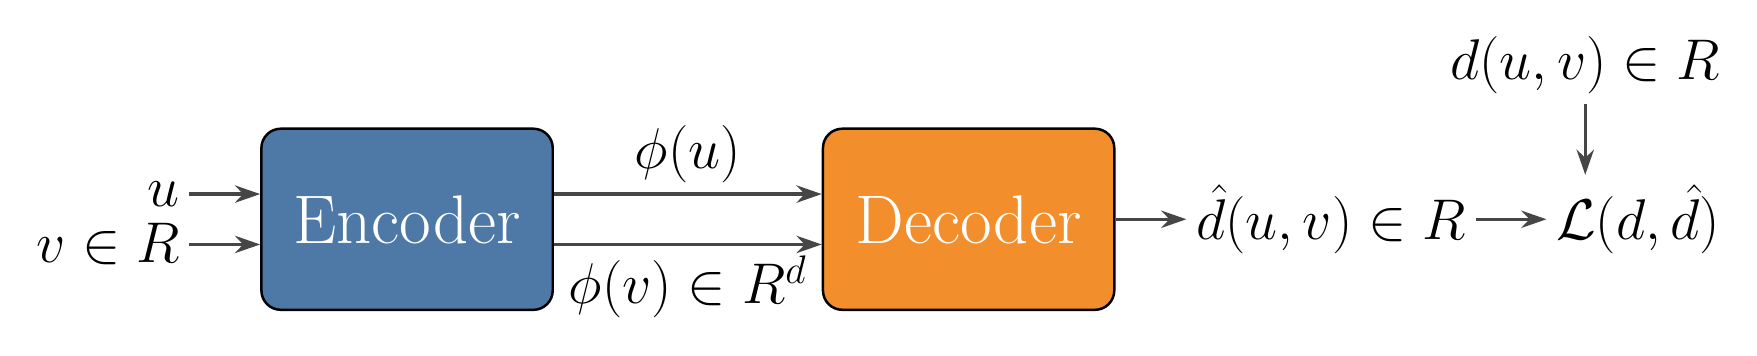
\begin{tikzpicture}[
    box/.style={rectangle, rounded corners=7pt, minimum width=3.7cm, minimum height=2.3cm,
                text=white, font=\Huge, align=center, draw=black, line width=0.9pt, inner sep=0pt},
    arrow/.style={-{Stealth[length=3.2mm, width=2.2mm]}, very thick, gray!55!black},
    lbl/.style={font=\huge, text=black}
]

\node[box, fill=mgBaseline] (enc) {Encoder};
\node[box, fill=mgNN, right=3.4cm of enc] (dec) {Decoder};

% Inputs to encoder, on the same rails as the phi(u)/phi(v) arrows below
\node[lbl, left=\lblgap of enc.west, anchor=east, yshift=\railoffset] (u) {$u$};
\node[lbl, left=\lblgap of enc.west, anchor=east, yshift=-\railoffset] (v) {$v \in \mathbb{R}$};

\draw[arrow] (u) -- ([yshift=\railoffset]enc.west);
\draw[arrow] (v) -- ([yshift=-\railoffset]enc.west);

% Encoder -> Decoder, two labeled arrows, on the same rails as u/v above
\draw[arrow] ([yshift=\railoffset]enc.east) -- node[lbl, above] {$\phi(u)$} ([yshift=\railoffset]dec.west);
\draw[arrow] ([yshift=-\railoffset]enc.east) -- node[lbl, below] {$\phi(v) \in \mathbb{R}^d$} ([yshift=-\railoffset]dec.west);

% Decoder output
\node[lbl, right=\lblgap of dec] (dhat) {$\hat{d}(u,v) \in \mathbb{R}$};
\draw[arrow] (dec.east) -- (dhat.west);

\node[lbl, right=\lblgap of dhat] (loss) {$\mathcal{L}(d, \hat{d})$};
\draw[arrow] (dhat.east) -- (loss.west);

% Ground-truth distance feeding into the loss from above, right-aligned with loss
\node[lbl, anchor=south east] (dtrue) at ([yshift=\lblgap]loss.north east) {$d(u,v) \in \mathbb{R}$};
\draw[arrow] (dtrue.south) -- (dtrue.south |- loss.north);

\end{tikzpicture}
\end{document}
